%%%%%%%%%%%%%%%%%%% vorlage.tex %%%%%%%%%%%%%%%%%%%%%%%%%%%%%
%
% LaTeX-Vorlage zur Erstellung von Projekt-Dokumentationen
% im Fachbereich Informatik der Hochschule Trier
%
% Basis: Vorlage svmono des Springer Verlags
%
%%%%%%%%%%%%%%%%%%%%%%%%%%%%%%%%%%%%%%%%%%%%%%%%%%%%%%%%%%%%%

\documentclass[envcountsame,envcountchap, deutsch]{i-studis}

\usepackage{makeidx}         	% Index
\usepackage{multicol}        	% Zweispaltiger Index
%\usepackage[bottom]{footmisc}	% Erzeugung von Fu�noten

%%-----------------------------------------------------
%\newif\ifpdf
%\ifx\pdfoutput\undefined
%\pdffalse
%\else
%\pdfoutput=1
%\pdftrue
%\fi
%%--------------------------------------------------------
%\ifpdf
\usepackage[pdftex]{graphicx}
\usepackage{epstopdf}
\usepackage[pdftex,plainpages=false]{hyperref}
%\else
%\usepackage{graphicx}
%\usepackage[plainpages=false]{hyperref}
%\fi

%%-----------------------------------------------------
\usepackage{color}				% Farbverwaltung
%\usepackage{ngerman} 			% Neue deutsche Rechtsschreibung
\usepackage[english, ngerman]{babel}
%\usepackage[latin1]{inputenc} 	% Erm�glicht Umlaute-Darstellung
\usepackage[utf8]{inputenc}  	% Erm�glicht Umlaute-Darstellung unter Linux (je nach verwendetem Format)

%-----------------------------------------------------
\usepackage{listings} 			% Code-Darstellung
\lstset
{
	basicstyle=\scriptsize, 	% print whole listing small
	keywordstyle=\color{blue}\bfseries,
								% underlined bold black keywords
	identifierstyle=, 			% nothing happens
	commentstyle=\color{red}, 	% white comments
	stringstyle=\ttfamily, 		% typewriter type for strings
	showstringspaces=false, 	% no special string spaces
	framexleftmargin=7mm, 
	tabsize=3,
	showtabs=false,
	frame=single, 
	rulesepcolor=\color{blue},
	numbers=left,
	linewidth=146mm,
	xleftmargin=8mm
}
\usepackage{textcomp} 			% Celsius-Darstellung
\usepackage{amssymb,amsfonts,amstext,amsmath}	% Mathematische Symbole
\usepackage[german, ruled, vlined]{algorithm2e}
\usepackage[a4paper]{geometry} % Andere Formatierung
\usepackage{bibgerm}
\usepackage{array}
\hyphenation{Ele-men-tar-ob-jek-te  ab-ge-tas-tet Aus-wer-tung House-holder-Matrix Le-ast-Squa-res-Al-go-ri-th-men} 		% Weitere Silbentrennung bei Bedarf angeben
\setlength{\textheight}{1.1\textheight}
\pagestyle{myheadings} 			% Erzeugt selbstdefinierte Kopfzeile
\makeindex 						% Index-Erstellung


%--------------------------------------------------------------------------
\begin{document}
%------------------------- Titelblatt -------------------------------------
\title{Audio Plugin: Delay Effekt}
%\subtitle{English Title}
%---- Die Art der Dokumentation kann hier ausgew�hlt werden---------------
%\project{Bachelor-Projektarbeit}
%\project{Tool- und Pluginprogrammierung}
%\project{Master-Projektstudium}
%\project{Master-Abschlussarbeit}
%\project{Seminar zur Vorlesung ...}
\project{Hausarbeit zur Vorlesung Tool- und Plugin-Programmierung}
%--------------------------------------------------------------------------
%\supervisor{Prof. Dr. C. Rezk-Salama} 		% Betreuer der Arbeit
\author{Simon Steiner} 							% Autor der Arbeit
\address{Trier,} 							% Im Zusammenhang mit dem Datum wird hinter dem Ort ein Komma angegeben
\submitdate{28.2.2019} 				% Abgabedatum
%\begingroup
%  \renewcommand{\thepage}{title}
%  \mytitlepage
%  \newpage
%\endgroup
\begingroup
  \renewcommand{\thepage}{Titel}
  \mytitlepage
  \newpage
\endgroup
%--------------------------------------------------------------------------
\frontmatter 
%--------------------------------------------------------------------------
%\preface

Ein Vorwort ist nicht unbedingt nötig. Falls Sie ein Vorwort schreiben, so ist dies der Platz, um z.B. die Firma vorzustellen, in der diese Arbeit entstanden ist, oder einigen Leuten zu danken, die in irgendeiner Form positiv zur Entstehung dieser Arbeit beigetragen haben. Auf keinen Fall sollten Sie im Vorwort die Aufgabenstellung näher erläutern oder vertieft auf technische Sachverhalte eingehen.				% Vorwort (optional)
\kurzfassung

%% deutsch
\paragraph*{}
Wie werden Signale mit einem Audio-Plugin verzögert wiedergegeben? Dies wird in dieser Ausarbeitung genauer behandelt. Dabei wird eine neue Klasse erstellt die all dies übernimmt. Ein wichtiges Konzept ist dabei ein Kreisspeicher der am Ende wieder von vorne beginnt. 
Ein ansprechendes UI sowie angenehme Interaktionen damit sind auch ein wichtiger Punkt, den ein Produzent arbeitet bei fast jedem Lied mit Delayplugins. 			% Kurzfassung Deutsch/English
\tableofcontents 						% Inhaltsverzeichnis
%\listoffigures 							% Abbildungsverzeichnis (optional)
%\listoftables 							% Tabellenverzeichnis (optional)
%--------------------------------------------------------------------------
\mainmatter                        		% Hauptteil (ab hier arab. Seitenzahlen)
%--------------------------------------------------------------------------
% Die Kapitel werden in separaten .tex-Dateien abgelegt und hier eingebunden.
\chapter{Einleitung und Motivation}

Musik findet sich überall im Alltag. Sei es im Einkaufszentrum oder auf dem Smartphone. Doch wie wird eins dieser Lieder produziert. 
Jede Person mit einem Computer kann heutzutage Musik damit erzeugen. Anwendungen, die dies können, sind weit verfügbar und in verschiedenen Preisklassen erhältlich. Ein persönlicher Favorit ist Ableton Live. Diese digitalen Workstations enthalten oftmals mehrere digitale Instrumente und Effekte. Ein beliebter Effekt ist das verzögerte Wiedergeben von den erzeugten Tönen wie zum Beispiel das Rufen in den Bergen (''Wer ist der Bürgermeister von Wesel''). Dies wird oftmals als Delay Effekt bezeichnet. Ein bekanntes Lied, was diesen Effekt benutzt hat, ist \textit{The Police - Every Breath You Take}.

Das Ziel dieser Arbeit ist es ein funktionierendes Delay Plugin für Ableton Live zu erstellen. Zum dem sollte es auch das verzögerte Audiosignal mehrmals wiederholen und dabei leiser werden. Mit Hilfe eines Reglers lässt sich das Mischverhältnis zwischen verzögertem Audiosignal und originalem Input verändern.
\chapter{Allgemein}

%(Separate) Dokumentation notwendig
%formlos 5-10 Seiten
%Thema, Motivation, ggf. Bedienung des Programms
%Begründung der wichtigen Design-Entscheidungen bei der Umsetzung

% Allg. Text bezueglich Juce und PLuginFormaten

Um Musik am Computer zu produzieren werden verschiedene Synthesizer und Effekte benutzt. Diese sind oftmals in C++ programmiert. Wichtig ist hierbei die Unterstützung von dem Musikprogrammen (Ableton Live) und das Wissen über verschiedene Plugin Formate.

\section{JUCE}

Juce ist ein C++ Framework zur Erstellung von Desktop und mobilen Anwendungen. Das Framework ist Open-Source und kann von dem GitHub-Repository heruntergeladen werden. Dort sind verschiedene Wrapper-Klassen enthalten die es ermöglichen, Audio Anwendungen zu erstellen \cite{JUCE}. 

Die Besonderheit von Juce bildet das Tool Projucer. Dieses Tool ist eine IDE zum Erstellen und Verwalten von Juce Projekten. Mit ein paar Klicken erstellt dieses Tool für jede gewünschte Plattform ein Projekt. Zum Beispiel kann eingestellt werden, dass ein Visual Studio 2017 und ein XCode Projekt erstellt werden kann. Bei Projekte verwenden den selben Sourcecode. In den Projekten selber werden, je nach Auswahl, weitere Projekte erzeugt abhängig davon, welche Plugin Formate erstellt werden sollen.

\begin{figure}
	\centering
	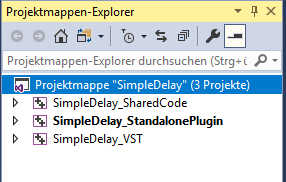
\includegraphics[width=0.7\linewidth]{images/projektmappe}
	\caption{VS '17 Projektmappen-Explorer. Erstellen des Projekts erzeugt hier ein .exe und ein VST2 Plugin (.dll)}
	\label{fig:projektmappe}
\end{figure}

Der Projucer erzeugt ein kleines Programmcodeskelett mit nützlichen Standardfunktionen. Dies vereinfacht den Einstieg, so dass nicht viel Zeit mit der Einarbeitung von irgendwelchen SDKs verschwendet wird.

\section{Plugins}

%Formate
In der heutigen Musikproduktion werden verschiedene Formatstandards für Plugins eingesetzt. Die Wahl für einen gewissen Standard ist abhängig von dem gewählten Betriebssystem sowie welche digitale Audioworkstation (DAW) verwendet wird. Um festzustellen, welche Formate von der jeweiligen DAW unterstützt wird, sollte die Herstellerwebseite bezogen werden. Die Formate unterscheiden sich in ihrer Funktion nicht großartig. Dazu eine kleine Liste von bekannten Formaten und unterstützenden DAWs \cite{PF}:

\begin{itemize}
	\item VST (Virtual Studio Technology): Ableton Live, Fl Studio, Cubase, Reason, Reaper
	\item AU (Audio Unit)[Nur Mac]: Ableton Live, Logic Pro, Studio One 
	\item RTSA (Real Time AudioSuit): Pro Tools
	\item AAX (Avid Audio eXtension): Pro Tools
\end{itemize}

Steinberg stellt zur Erstellung von VSTs ein SDK bereit. Im Moment beginnt bei Steinberg eine Umstellung von dem VST2 Standard auf den VST3 Standard. In der aktuell verfügbaren SDK gibt es keine Unterstützung mehr für die Erstellung von VST2 Plugins. Manche Hersteller haben sich noch nicht angepasst wie zum Beispiel Ableton, diese akzeptieren bislang noch keine VST3 Plugins. Ältere Versionen von Juce haben noch einen VST2 Support zum Erstellen von Plugins. Die aktuelle Version kann jedoch nur noch den neusten VST Standard erzeugen.
Da zum Testen stand nur Ableton zu Verfügung, weshalb das Plugin mit einer älteren Version von Juce erstellt werden musste. Das Plugin selber ist eine .dll-Datei, welche sich im VST-Plugin Ordner der DAW befinden muss. Wichtig ist, dass das Plugin und die DAW die selbe Bit-Architektur haben (32/64).
\chapter{Konzept und Theorie}
%Oberflaeche erklären und was passiert

Die Umsetzung des Delay Plugins besteht aus zwei Teilen: Das Delay und die Steuerung der Parameter mit Hilfe einer GUI.

\section{Delay Effekt}

Der Delay Effekt ist im Grunde eine Wiederholung des Eingangsignals zu einer späteren Zeit (siehe \ref{fig:ableton}: Spur 2). Da zu einem späteren Zeitpunkt dieses exakte Signal nicht mehr da ist muss es in einem Buffer gespeichert werden. Zur Vereinfachung wird der Buffer wie ein kreisförmiger Speicher gesehen. Mit Hilfe von dem Modulo-Operator ist dies programmiertechnisch möglich.
Sollte zu einem bestimmten Zeitpunkt das vergangene Signal zum aktuellen Input hinzugefügt werden, so muss eine gewisse Anzahl an Samples im Speicher zurückgesprungen werden. Dies lässt sich mit Hilfe der Samplerate berechnen.
Um dieses Signal nicht nur einmal wiederzugeben sondern langsam abschwächen zu lassen (siehe \ref{fig:ableton}: Spur 3) muss das verzögerte Signal wieder in den Delaybuffer eingespeist werden.

\begin{figure}
	\centering
	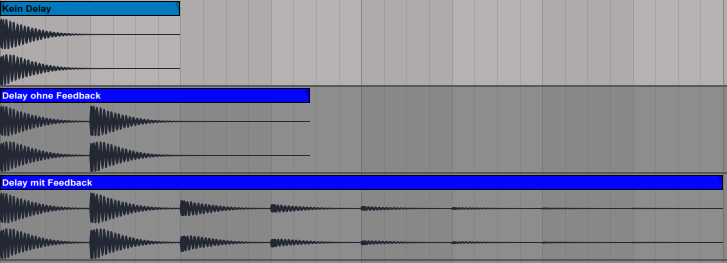
\includegraphics[width=0.8\linewidth]{images/ableton}
	\caption{Ausschnitt aus Ableton Live bei Anwendung des Delay Plugins. 3 verschiedene Audiospuren. 1. Spur: Nur das original Signal. 2. Spur: Signal wird nach 500ms wiederholt. 3. Spur: Wiederholung des Signals mit Einspeisung des verzögerten Signals aber immer leiser werdend. [Siehe Anlage Audio 1 bis 3]}
	\label{fig:ableton}
\end{figure}

Als Veranschaulichung dient hierbei Abbildung \ref{fig:delayline}. Hier werden N Samples direkt vom Input an den Output weitergeleitet als auch im DlyWBuf gespeichert. Das verzögerte Signal \textit{g} wird zusammen mit dem Input addiert und befindet sich dann im Output. \textit{fb} entspricht dem selben Signal wie \textit{g} und wird gleichzeitig mit dem aktuellen Input im Delaybuffer gespeichert.

\begin{figure}
	\centering
	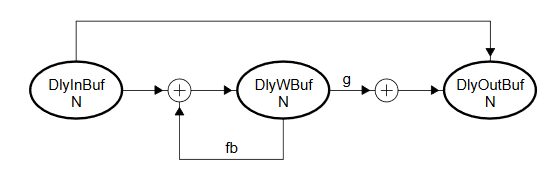
\includegraphics[width=0.7\linewidth]{images/delayline}
	\caption{Ablaufdiagramm einer typischen Delayline mit Feedback. Input landet direkt im Output. Input wird gleichzeitig im Delaybuffer gespeichert. Verzögertes Signal wird zusammen mit Input im Output zusammengeführt. Gleichzeitig wird das verzögerte Signal wieder im Delaybuffer eingespeist. \cite{HTC}}
	\label{fig:delayline}
\end{figure}


\section{GUI}

Es gibt bei dieser Art von Delay 3 Werte die verändert werden könnten. Eine mögliche Umsetzung wäre das Nutzen von 3 Slidern. Einen für den Verzögerungswert (Delaytime), Feedback und Mischverhältnis. Für zukünftige Plugins ist jedoch die Verwendung eines Felds, wo Werte abhängig von einer Position auf der x- und y-Achse sind, von nutzen. 
Slider sind in dem Framework schon standardmäßig dabei, zusammen mit dazugehörigen Observer-Pattern. Zur Anzeige der Werte kann bei dem Slider eine zugehörige TextBox (TextEditor) aktiviert werden.

Das ControlPad muss jedoch selbst umgesetzt werden. Es besteht aus einem Kontrollpunkt (Trackball). Der Mittelpunkt des Trackballs darf nicht das darunterliegende Feld verlassen. Um die Werte anzuzeigen, welche die jeweilige Achsenposition repräsentieren, gibt es noch zwei TextBoxen (xValue, yValue). Alles zusammen ergibt das Element \textit{ControlPad }.

Das Hintergrundbild wirkt als Anlehnung an das Echo in den Bergen. 

\begin{figure}
	\centering
	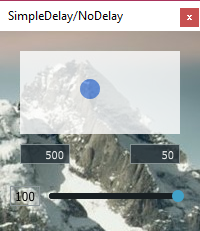
\includegraphics[width=0.5\linewidth]{images/plugininableton}
	\caption{}
	\label{fig:plugininableton}
\end{figure}



\chapter{Implementierung}

%Codebrocken erklären


\section{Delay Processing}

Das wichtigste in der digitalen Signalverarbeitung ist die Methode \textit{processBlock()}. In dieser Methode findet die ganze Signalbearbeitung statt. Im AudioBuffer Objekt stehen die aktuellen Eingangsamples. Diese werden immer blockweise geladen. Dieser AudioBuffer ist zeitgleich auch der Ausgangsbuffer.

Der Nachfolgende Code ist des Herzstück des Delay Plugins. Hier werden die aktuellen Samples in den Delaybuffer des Objekts \textit{d} gespeichert. Dann wird in ein AudioBuffer-Objekt die vergangenen Samples aus dem Delaybuffer kopiert. Die darin enthaltenen Samples werden mit einer gewissen Lautstärke (Feedbackwert) zu den vorhandenen Samples in dem Delaybuffer aufaddiert (nicht ersetzt!) aber an der selben Stelle wie vorher die Eingangssamples gespeichert wurden. Alle vergangen Samples erhalten noch eine gewisse Lautstärke (Mixwert). Am Ende werden die vergangenen Samples im AudioBuffer-Objekt zu den Eingangssamples aufaddiert.

\begin{lstlisting}[language=C++, caption=Ausschnitt aus processBlock()]
for (int channel = 0; channel < totalNumInputChannels; ++channel)
{
float* inputData = buffer.getWritePointer (channel);

d.setBufferData(channel, inputNumSamples, inputData);

float delayTimeVal = *parameters->getRawParameterValue("timeID");

d.getBufferData(channel, inputNumSamples,delayTimeVal, delayedSignal);

float feedbackVal = *parameters->getRawParameterValue("feedbackID");

d.addFeedbackData(channel, inputNumSamples,
	feedbackVal/100.0f, delayedSignal.getReadPointer(channel));

float mixVal = *parameters->getRawParameterValue("mixID");
delayedSignal.applyGain(mixVal/100.0f);

buffer.addFrom(channel, 0, delayedSignal, channel, 0, inputNumSamples);

}
\end{lstlisting}

Nach der Schleife ist es nur wichtig mit der Methode \textit{updateBufferPos()} aufzurufen um die Schreibposition zu verschieben.

Alle Operationen die auf dem Delaybuffer (Kreisspeicher) arbeiten befinden sich im Delay-Objekt. Jede diese Operationen verschiebt aber nicht die Samples einzeln in den Delaybuffer sondern mit Hilfe von Vektorfunktionen. Andernfalls wird die Laufzeit möglicherweise beeinflusst und zwar auf die schlechte Art.

Das einzige Problem an dieser Implementierung ist, wenn die Delaytime geändert wird, entstehen Artefakte. Dies kommt daher, dass sich die Position zum lesen der vergangenen Samples geändert hat. Damit entsteht zwischen dem alten und  neuen Wert ein zu großer Unterschied den der Lautsprecher nicht natürlich wiedergeben kann. Daraus folgt ein Knackgeräusch. Dies könnte mit Hilfe von Interpolation entfernt werden.

\section{ControlPane}

Die ControlPane-Klasse war als langfristige Erweiterung geplant. Diese könnte zum Beispiel für eine Implementierung eines Filters mit Resonanz genutzt werden. Dafür wurden Vorkehrungen bei der Implementierung von Methoden gewählt.

Die Wertebereichslimits können auch so gesetzt werden, dass der Minimalwert negativ sein kann. Die Methoden zur Umrechnung von Achspositionen zu Absolutwerten (\textit{convertAxisToValue()}) und umgekehrt von Absolutwert zu Achsenposition (\textit{convertValueToAxis()}) berechnen korrekte Werte egal ob der Anfangswert negativ ist. Solche Berechnungen, welche Werte von einem bestimmten Bereich auf einen anderen ableitet, sind ein persönlicher Favorit von mir. 

Das der Trackball über das Feld hinausgehen kann wirkt auf den User besser. Könnte der Trackball sich nicht hinaus bewegen, so wirkt der Trackball nicht als rundes Objekt sondern eher als Quadrat. Damit bleibt die Illusion erhalten das es wirklich ein rundes Objekt ist. Zu dem wirkt es schöner wenn der Mittelpunkt des Trackballs an der Mausklick Position ist.
\chapter{Bedienungsanleitung}

%Optional, je nachdem wie sich Ausarbeitung entwickelt

Es lassen sich Delaytime (Zeit, die verstreicht in Millisekunden bis das Signal wiederholt wird), Feedback (Lautstärkewert, mit der das wiederholte Signal wieder in den Delaybuffer eingespeist wird) und das Mischverhältnis im Output zwischen Inputsignal und dem Signal aus dem Delaybuffer.

Ist das Mischverhältnis auf 0 Prozent, so wird nur das Eingangssignal ausgegeben. Je höher das Mischverhältnis des mehr wird von dem verzögerten Signal gehört. Bei 100 Prozent ist Eingangssignal und das verzögerte Signal gleich laut.

Das Verschiebung des Trackballs auf der x-Achse verändert die Zeit bis das Signal wiederholt wird. Mit diesem Plugin ist eine Zeit zwischen 100ms und 1000ms möglich.

Das Verschieben des Trackballs auf der y-Achse verändert die Lautstärke des wiederholenden Signals. Es ist nicht möglich den Wert auf 100 zu setzen, da das Signal sonst ewig wiederholt wird.

Im Ordner \textit{Audio} liegen 3 Beispiele. Eines ohne Delay, eines mit einem 500ms Delay und das selbe noch einmal nur mit Feedback.

Im Ordner \textit{Dateien} liegen eine eigenständige Anwendung und eine .dll zur Verwendung in DAWs.


\section{Plugin}

Um das erstellte Plugin in einer DAW zu verwenden:

\begin{itemize}
	\item Projekt erstellen. Damit wird eine .dll erzeugt
	\item Aus ../Projektordner/Builds/VisualStudio2017/Win32/Debug/VST die Datei mit der Endung \textit{.dll} in den VSTPlugin Ordner der DAW ziehen und neu scannen lassen
	\item Sollte es dort nicht gefunden werden, kann die Bit-Architektur des DAW/Plugin ungleich sein. Lösung: Plugin mit einer anderen Architektur erstellen
	\item Plugin nach einem digitalem Instrument platzieren und an den Reglern die Werte verändern
\end{itemize}

\section{Standalone}

Achtung: Bei Verwendung einer Lautsprecheranlage kann es zu Rückkopplungen kommen.

Die eigenständige Datei (.exe) starten. Es können möglicherweise Dateien (.dll) fehlen um die Datei auszuführen. Nach Installation der fehlenden Datei sollte auch die Standalone Variante funktionieren. 
\chapter{Zusammenfassung und Ausblick}

Mit dem JUCE Framework ist es möglich ein Delay Plugin zu erstellen. Dieses funktioniert ohne Knackgeräusche wenn während der Nutzung der Delaytimewert nicht verändert wird. Folglich empfiehlt sich also nicht den Wert in einer DAW zu automatisieren. 

Die Erstellung eigener UI-Komponenten ist auch relativ einfach möglich. Diese können entweder aus weiteren vorgefertigten Elementen bestehen oder eigene zeichnen wie in diesem Fall den Trackball und das Begrenzungsfeld.

Diese Variante könnte in der Zukunft weiter optimiert (Interpolation) oder um weitere Funktionen erweitert werden. Eine mögliche Erweiterung ist ein unterschiedliches Delay pro Kanal, so dass einer eine Verzögerung von 500ms und der andere von 550ms hat.
% ...
%--------------------------------------------------------------------------
\backmatter                        		% Anhang
%-------------------------------------------------------------------------
\bibliographystyle{geralpha}			% Literaturverzeichnis
\bibliography{literatur}     			% BibTeX-File literatur.bib
%--------------------------------------------------------------------------
\printindex 							% Index (optional)
%--------------------------------------------------------------------------
\begin{appendix}						% Anh�nge sind i.d.R. optional
   %\chapter{Glossar}

\abbreviation{DisASTer}		{DisASTer (Distributed Algorithms Simulation Terrain), A platform for the Implementation of Distributed Algorithms}
\abbreviation{DSM}			{Distributed Shared Memory}
\abbreviation{AC}			{Linearisierbarkeit (atomic consistency)}
\abbreviation{SC}			{Sequentielle Konsistenz (sequential consistency)}
\abbreviation{WC}			{Schwache Konsistenz (weak consistency)}
\abbreviation{RC}			{Freigabekonsistenz (release consistency)}
			% Glossar   

\end{appendix}

\end{document}
